

\documentclass[../../tc_tp3_main.tex]{subfiles}

\begin{document}
\chapter{Control de tonos y ecualizador de fase}
\todo{introduccion al tema}

\begin{figure}[H]
\centering
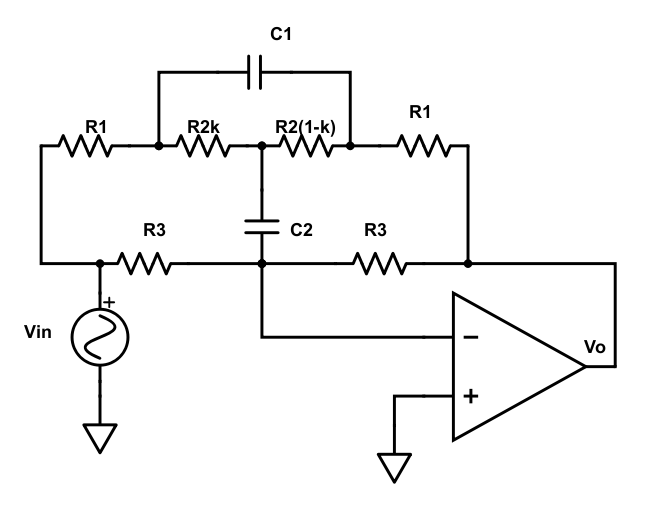
\includegraphics[width=0.3\textwidth]{imagenes/circuitoControlTonos.png}
\caption{Circuito del control de tonos} \label{fig:cct}
\end{figure}




\section{Función transferencia}

Para hallar la función transferencia $H(S)=\frac{V_{o}}{V_{in}} $del circuito de la figura \ref{fig:cct}, se realizaron transformaciones estrella a triangulo y viceversa, reduciendo el circuito. Dichas transformaciones se realizaron con Matlab.



\begin{figure}[H]
\centering
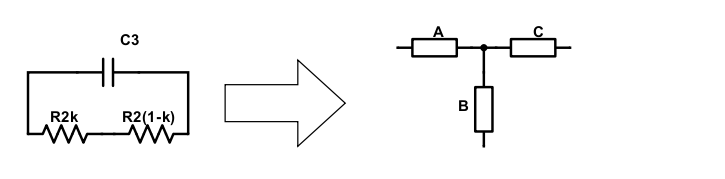
\includegraphics[width=0.5\textwidth]{imagenes/simpl1.png}
\caption{Transformación triangulo a estrella} \label{fig:cs1}
\end{figure}

Reemplazando el circuito triangulo por el estrella, permitio agrupar $A$ con $R_1$, $C$ con$ R_1$ y$ B$ con $C_1$. Obteniendo un nuevo circuito estrella con las siguientes impedancias $ K_1$ , $K_2$ y  $K_3$, tal como se observa en la figura \ref{fig:cs2}.

\begin{gather}
   A=\frac{K\, R_{2}}{C_{1}\, S\, \left(\frac{1}{C_{1}\, S} - R_{2}\, \left(K - 1\right) + K\, R_{2}\right)} \\
B=-\frac{R_{2}\, \left(K - 1\right)}{C_{1}\, S\, \left(\frac{1}{C_{1}\, S} - R_{2}\, \left(K - 1\right) + K\, R_{2}\right)}\\
C=-\frac{K\, {R_{2}}^2\, \left(K - 1\right)}{\frac{1}{C_{1}\, S} - R_{2}\, \left(K - 1\right) + K\, R_{2}}
\end{gather}


\begin{figure}[H]
\centering
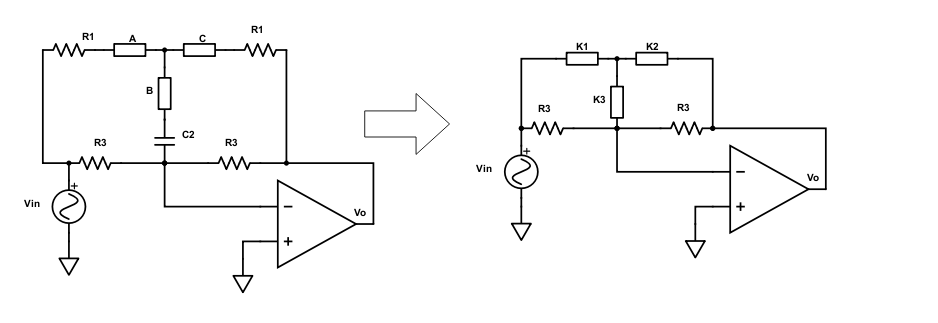
\includegraphics[width=0.5\textwidth]{imagenes/simpl2.png}
\caption{Agrupo impedancias en serie} \label{fig:cs2}
\end{figure}


\begin{figure}[H]
\centering
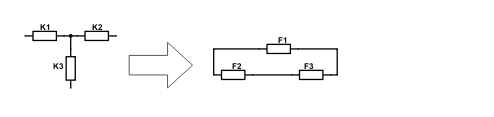
\includegraphics[width=0.5\textwidth]{imagenes/simpl3.png}
\caption{Transformación estrella a triangulo} \label{fig:cs3}
\end{figure}

Dicho circuito estrella se lo transformó a triangulo para de esta manera poder agrupar $F_2$ con $R_3$ y $F_3$ con $R_3$ (figura \ref{fig:cs4}).




\begin{figure}[H]
\centering
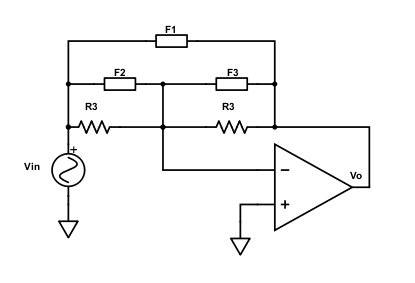
\includegraphics[width=0.5\textwidth]{imagenes/simpl4.png}
\caption{Agrupo impedancias en paralelo} \label{fig:cs4}
\end{figure}



\begin{figure}[H]
\centering
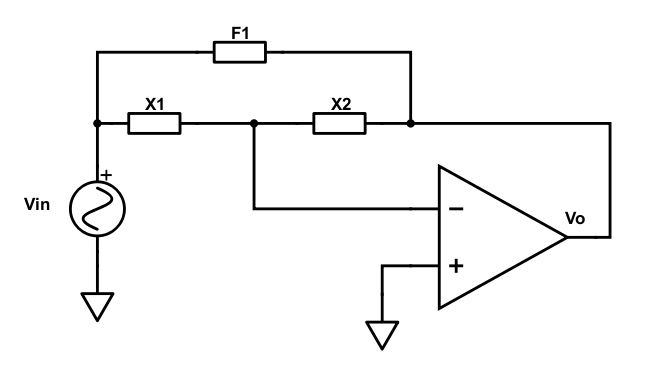
\includegraphics[width=0.5\textwidth]{imagenes/simplFin.png}
\caption{Circuito equivalente} \label{fig:csFin}
\end{figure}

Finalmente se obtiene el circuito de la figura \ref{fig:csFin}. Considerando que el OpAmp se comporta idealmente y la corriente que circula internamente por la entrada del amplificador es cero, resulta la siguiente  función transferencia:

\begin{equation}
H(S)=- \frac{X_2}{X_1}\label{eq:circuitoRed}
\end{equation}

Donde
\todo{ver que pasa con las ecuaciones} 
\begin{gather}
X_1=    \\
X_2=
\end{gather}

Aplicando las siguientes condiciones de diseño sobre la función transferencia
\begin{gather}
 R_3 >> R_1   \\
 R_3 =10 R_2   \\
C_1=10C_2
\end{gather}

Obtenemos

\todo{ecuacion reducida}

Si
\begin{equation}
-20C_{2}^2 K^2 R_{2}^2 R_{1}  S^{2} + 20 C_{2}^{2} K R_{1} R_{2}^2+ 10 C_{2}^2 R_{1}^2 R_{2} S^{2} + 100 C_{2}^{2} R_{1} R_{2}^2 S^{2} \approx 100 C_{2}^2 R_{1} R_{2} ^2 S^2
\end{equation}

\todo{ecuacion reducida} 

La ecuacion xx posee la forma

\begin{equation}
H(S)=\frac {\left( \frac{S}{W_0} \right) ^2 + \frac{S}{Q_Z W_0} +1}{\left( \frac{S}{W_0} \right) ^2 +\frac{S}{Q_Z W_0}+1}
\end{equation}

Dicha funsión transferencia corresponde a un circuito pasa banda de segundo orden, donde $W_0$ es la fecuencia central de la banda y 






\end{document}
